 \documentclass{report}
 
\usepackage[utf8]{inputenc} 
\usepackage[T1]{fontenc}      
\usepackage[top=2.0cm, bottom=3cm, left=3.0cm, right=3.0cm]{geometry}
\usepackage{graphicx}
\usepackage{wrapfig}
\usepackage{amsmath,esint }
\usepackage{amssymb}
\graphicspath{{figures/}{../figures}}

\newcommand*\dif{\mathop{}\!\mathrm{d}}
\newcommand*\diver{\mathop{}\!\mathrm{div}}
\newcommand*\grad{\mathop{}\!\mathrm{grad}}

\begin{document}

\section*{Puits de potentiel assymétrique $\bullet\bullet\circ$}

On considère une particule de masse $m$ et d'énergie $E$ piégée dans un puit de potentiel comme représenté ci-dessous :

\begin{figure}[h!]
\centering
  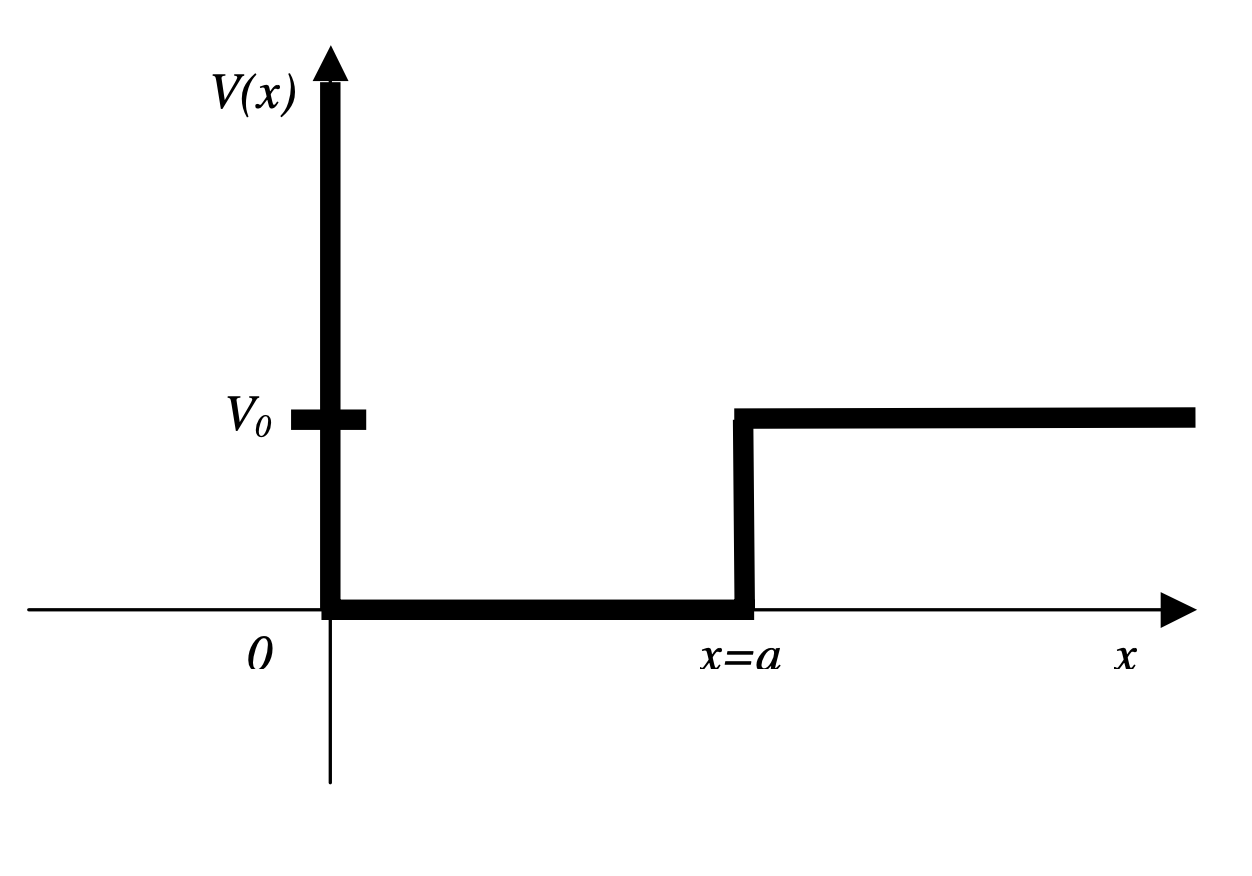
\includegraphics[width=0.6\textwidth]{puits_assy.png}
\end{figure}

On ne s'intéresse qu'au mouvement unidimentionnel de la particule suivant $x$. On cherche un état stationnaire de l'équation de Schrödinger de la forme $\Psi(x,t)=\psi(x)e^{-iEt/\hbar}$

\begin{itemize}

	\item[$\clubsuit$] Montrer que, malgré la discontinuité de $V$ en $x=a$, $\psi$ et sa dérivée sont continues.
	
	\item[$\clubsuit$] Montrer que pour $E<V_0$, la fonction d'onde pour un état lié, ou localisé dans le puit, s'écrit :
	\begin{align*}
		\psi(x,t)&=A\sin(qx)\quad \mathrm{si}\quad 0<x<a \\
		\psi(x)&=Be^{-x/x_0}\quad \mathrm{si}\quad x>a \\
	\end{align*}
avec $E=\hbar^2q^2/2m$ et $x_0=\hbar/\sqrt{2m(V_0-E)}$. On ne demande pas de donner l'expression des constantes $A$ et $B$.

	\item[$\clubsuit$] La solution met en évidence une longueur caractéristique $x_0$, proposer une interprétation physique. Existe t-il une longueur équivalente pour une particule matérielle clasique ? Donner un exemple de longueur analogue dans un autre domaine de la physique. 
	
	\item[$\clubsuit$] Utiliser les conditions aux limites pour en déduire que le vecteur d'onde $q$ doit satisfaire à la relation :
	\begin{align*}
	 \mathrm{cotan}(y)=-\frac{\sqrt{\gamma^2-y^2}}{y}
	\end{align*}
avec $y=qa$ et $V_0=\hbar^2\gamma^2/2ma^2$.

\item[$\clubsuit$] Tracer qualitativement les solutions graphiques de cette équation. En déduire qu'il n'existe aucun état lié pour des valeurs de $V_0$ inférieures à un seuil $W$ que l'on exprimera. 

\end{itemize}

\newpage

\section*{Etats stationnaire d'une particule dns un puits de profondeur finie $\bullet\bullet\circ$}

Une particule de masse $m$ et d'énergie $E$ (avec $-V_0<E<0$) est confinée dans un puits de largeur $2a$ et de profondeur $-V_0$. L'énergie potentielle de la particule prend alors la forme :
\begin{align*}
	\mathrm{(1) :}\quad V(x)&=0\quad \mathrm{pour}\quad x<-a \\
		\mathrm{(2) :}\quad V(x)&=-V_0\quad \mathrm{pour}\quad -a<x<a \\
		\mathrm{(3) :}\quad V(x)&=0\quad \mathrm{pour}\quad x>a \\
\end{align*}

On note $\Psi(x,t)=\phi(x)e^{-iEt/\hbar}$ la fonction d'onde pour un état stationnaire d'énergie $E$ de la particule confinée dans ce puits. 

\begin{itemize}

	\item[$\ast$] Etablir les équations différentielles vérifiées par la fonction $\phi(x)$ dans les différentes régions de potentiel (on notera la fonction d'onde $\phi_n(x)$ pour la région $n=1$, 2 ou 3). 
	
	\item[$\ast$] En déduire que $\phi_1(x)=A_1e^{\alpha x}$, $\phi_2(x)=A_2e^{ik x}+B_2e^{-ik x}$ et $\phi_3(x)=A_3e^{-\alpha x}$, en précisant les expressions de $\alpha$ et $k$. Etablir le système d'équations vérifiées par $A_1$, $A_2$, $A_3$ et $B_2$.

\end{itemize}

La parité du potentiel permet d'affirmer que les fonctions $\phi(x)$ décrivant les états stationnaires sont paires (modes symétriques) ou impaires (modes antisymétriques). 

\begin{itemize}

	\item[$\ast$] Etablir pour les modes symétriques la relation reliant les grandeurs $k$ et $\alpha$, puis celle reliant les variables adimensionnées $u=2mV_0a^2/\hbar^2$ et $\xi=ka$. Justifier à l'aide d'un tracé qu'il y a quantification des niveaux d'énergie de la particule. 
	
	\item[$\ast$]Même question pour les modes antisymétriques.
	
	\item[$\ast$] Le mode fondamental est-il symétrique ou antisymétrique ?

\end{itemize}

\end{document}